\documentclass[tikz,border=5pt]{standalone}
\usepackage{times}
\usepackage{amsmath,amssymb}
\usetikzlibrary{positioning,fit,arrows.meta,backgrounds,shapes.geometric,calc,shadows,decorations.pathreplacing}

\begin{document}
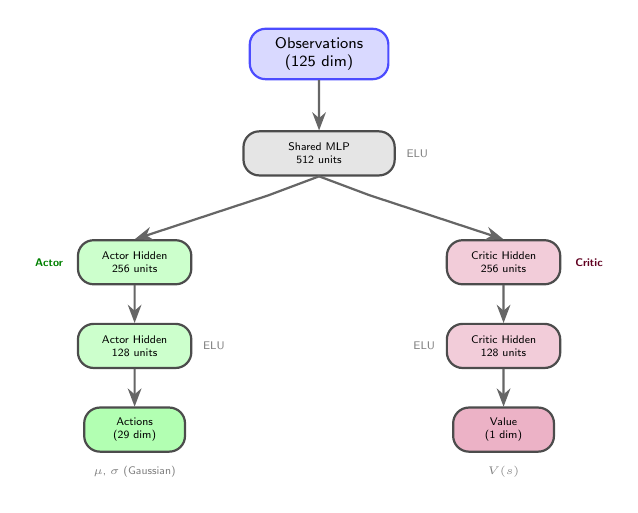
\begin{tikzpicture}[
    scale=0.8,
    transform shape,
    node distance=0.6cm,
    layer/.style={
        draw=black!70,
        rounded corners=2mm,
        minimum width=1.8cm,
        minimum height=0.7cm,
        font=\sffamily\tiny,
        thick,
        align=center
    },
    input/.style={
        draw=blue!70,
        fill=blue!15,
        rounded corners=2mm,
        minimum width=2.2cm,
        minimum height=0.8cm,
        font=\sffamily\scriptsize,
        thick,
        align=center
    },
    output/.style={
        draw=black!70,
        rounded corners=2mm,
        minimum width=1.6cm,
        minimum height=0.7cm,
        font=\sffamily\tiny,
        thick,
        align=center
    },
    arrow/.style={->, >=Stealth, thick, color=black!60}
]

% Input
\node[input] (obs) {Observations\\(125 dim)};

% Shared layers
\node[layer, fill=gray!20, below=0.8cm of obs, minimum width=2.4cm] (shared) {Shared MLP\\512 units};

% Split into actor and critic
\node[layer, fill=green!20, below left=1cm and 0.8cm of shared] (actor1) {Actor Hidden\\256 units};
\node[layer, fill=purple!20, below right=1cm and 0.8cm of shared] (critic1) {Critic Hidden\\256 units};

\node[layer, fill=green!20, below=0.6cm of actor1] (actor2) {Actor Hidden\\128 units};
\node[layer, fill=purple!20, below=0.6cm of critic1] (critic2) {Critic Hidden\\128 units};

% Outputs
\node[output, fill=green!30, below=0.6cm of actor2] (actions) {Actions\\(29 dim)};
\node[output, fill=purple!30, below=0.6cm of critic2] (value) {Value\\(1 dim)};

% Labels
\node[font=\sffamily\tiny\bfseries, green!50!black, left=0.1cm of actor1] {Actor};
\node[font=\sffamily\tiny\bfseries, purple!50!black, right=0.1cm of critic1] {Critic};

% Arrows
\draw[arrow] (obs) -- (shared);
\draw[arrow] (shared.south) -- ++(-0.8,-0.3) -- (actor1.north);
\draw[arrow] (shared.south) -- ++(0.8,-0.3) -- (critic1.north);
\draw[arrow] (actor1) -- (actor2);
\draw[arrow] (critic1) -- (critic2);
\draw[arrow] (actor2) -- (actions);
\draw[arrow] (critic2) -- (value);

% Activation annotations
\node[font=\sffamily\tiny, color=gray, right=0.05cm of shared.east] {ELU};
\node[font=\sffamily\tiny, color=gray, right=0.05cm of actor2.east] {ELU};
\node[font=\sffamily\tiny, color=gray, left=0.05cm of critic2.west] {ELU};

% Output annotations
\node[font=\sffamily\tiny, color=gray, below=0.1cm of actions] {$\mu$, $\sigma$ (Gaussian)};
\node[font=\sffamily\tiny, color=gray, below=0.1cm of value] {$V(s)$};

\end{tikzpicture}
\end{document}
